\title{Inverse Kinematics of a Continuum Stewart-Gough Robot}
\author{John Till}
\date{}

\documentclass[12pt]{article}

\usepackage[a4paper, margin=0.75in]{geometry}
\usepackage[colorlinks=true,urlcolor=blue]{hyperref}
\usepackage{amsmath,amssymb}
\usepackage{graphicx}

\usepackage{xcolor}
\definecolor{OffWhite}{rgb}{0.93,0.93,0.93}
\definecolor{QtCommentColor}{rgb}{0,0.5,0}
\definecolor{QtKeywordColor}{rgb}{0.5,0.5,0}
\definecolor{QtPurpleColor}{rgb}{0.5,0,0.5}
\definecolor{QtGlobal}{rgb}{0.808,0.361,0}
\definecolor{QtFunctionColor}{rgb}{0,0.404,0.486}

\usepackage[T1]{fontenc} %for upquotes in listings
\usepackage{textcomp} %for upquotes in listings
\usepackage{listings}
\lstset{
		language=C++,
		escapeinside={!-}{-!},
		upquote=true,
		%
		otherkeywords={Vector3d, DiagonalMatrix, VectorXd, Matrix3d, Map, MatrixXd, Vector6d, Vector2d,
									std, vector,
									UnitX, pow, inverse, transpose, segment, data, UnitZ, cross, hat,
									Zero, Identity, UnitY, cosseratRodOde, ode4, cols, row, main, shootingFunction,
									block, linear_rotation_error, solveLevenbergMarquardt, plot, Ones, cos, sin,
									Ry, initialize_StewartGough_pattern},
    morekeywords=[2]{Vector3d, DiagonalMatrix, VectorXd, Matrix3d, Map, MatrixXd, Vector6d, Vector2d,
		                 std, vector},
		morekeywords=[3]{UnitX, UnitZ, pow, inverse, transpose, segment, data, cross, hat,
		                 Zero, Identity, UnitY, cosseratRodOde, ode4, cols, row, main, shootingFunction,
										 block, linear_rotation_error, solveLevenbergMarquardt, plot, Ones, cos, sin,
										 Ry, initialize_StewartGough_pattern},
    %
		frame = single,
		rulecolor=\color{black},
    tabsize=4, % tab space width
    showstringspaces=false, % don't mark spaces in strings
		%
		basicstyle=\footnotesize,%\color{QtIdentifier},
		backgroundcolor=\color{OffWhite},
    commentstyle=\color{QtCommentColor}, % comment color
    keywordstyle=\color{QtKeywordColor}, % keyword color
		keywordstyle=[2]{\color{QtPurpleColor}},
		keywordstyle=[3]{\color{QtFunctionColor}},
    stringstyle=\color{QtCommentColor} % string color
}

\begin{document}

\makeatletter
\renewcommand{\@maketitle}{
\newpage
\null
\vskip 2em
\begin{center}
{\LARGE \@title \par}
\end{center}
\par
} \makeatother

\maketitle

Now that we have solved elastic rod problems, we can start combining rods to form continuum robots. In fact, we already have the necessary mathematical tools; the robot models will also be boundary value problems which we may solve with the shooting method. The main difference is an increase in complexity as we have multiple rods which are coupled together by constraint equations.

In this chapter, we solve the inverse kinematics for a continuum Stewart-Gough robot. This robot was introduced in the paper \href{https://ieeexplore.ieee.org/document/6906943}{``Toward Parallel Continuum Manipulators''} and considered in more detail through \href{https://ieeexplore.ieee.org/abstract/document/8207644}{``Parallel Continuum Robots: Modeling, Analysis, and Actuation-Based Force Sensing''}. The kinematics model is also described in chapter 3 of Caroline Bryson Black's dissertation, \href{https://trace.tennessee.edu/utk_graddiss/4443/}{``Modeling, Analysis, Force Sensing and Control of Continuum Robots for Minimally Invasive Surgery''}, which is freely available. The robot consists of six flexible rods extending through a baseplate and joining the end effector in the pattern of a \emph{Stewart-Gough platform} as shown below:
\begin{figure}[h]
	\centering
		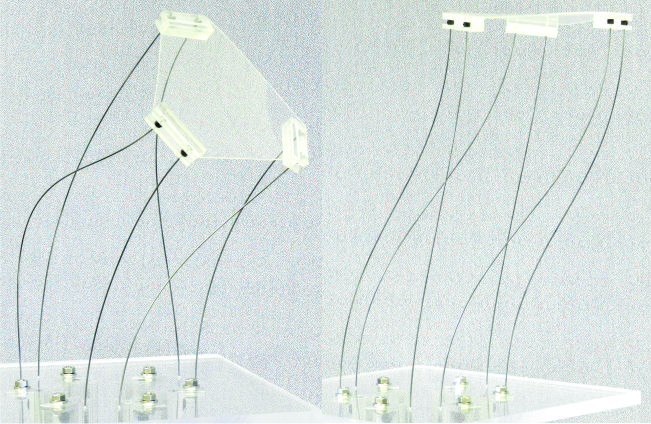
\includegraphics[width=0.80\textwidth]{fig/PCM.jpg}
	\label{fig:PCM}
\end{figure}

The robot is controlled by changing the length of each leg inserted through the base plate. The constraints to be satisfied are that the legs meet the end effector with the correct position and orientation, and that the static force balance of the end effector is satisfied. We will not consider the model equations in detail here; they are contained in the references listed above.

\newpage
We start the simulation script with parameters:
\begin{lstlisting}
//Independent Parameters
const double E = 200e9;
const double G = 80e9;
const double rad = 0.001;
const double rho = 8000;
const Vector3d g = -9.81*Vector3d::UnitZ();
const double ee_mass = 0.1;
const double scrib_R = 0.087; //radius of the hole pattern
const double alpha1 = 100*pi/180; //major angle of the hole pattern

//Dependent parameter calculations
const double A = pi*pow(rad,2);
const double I = pi*pow(rad,4)/4;
const double J = 2*I;
const DiagonalMatrix<double, 3> Kse = DiagonalMatrix<double, 3>(G*A,G*A,E*A);
const DiagonalMatrix<double, 3> Kbt = DiagonalMatrix<double, 3>(E*I,E*I,G*J);
const Vector3d F = ee_mass*g;
const Vector3d M = Vector3d::Zero();
const Vector3d pE = 0.4*Vector3d::UnitZ();
const Matrix3d RE = Ry(10*pi/180); //Bend 10 degrees above the y-axis
const double alpha2 = 120*pi/180 - alpha1; //minor angle of the hole pattern
\end{lstlisting}
We assume each of the six rods has the same parameters. The end effector mass ``ee\_mass'' is used when calculating the static force balance, and ``scrib\_R'' and ``alpha1'' define the hole pattern in the base plate and attachment pattern at the end effector.

We define an array ``p0'' which contains the position of each hole in the base plate and another array ``r'' which contains the translation from the end effector to the rod attachment points in the end effector frame. These are initialized in the following function:
\begin{lstlisting}
//Hexagonal Stewart-Gough hole pattern
static Vector3d p0[6];
static Vector3d r[6];
void initialize_StewartGough_pattern(){
    for(int i = 0; i < 6; i++){
        double theta_b = (-alpha2 + ((i+1) - (i+1)%2)*alpha2 + (i-i%2)*alpha1)/2;
        p0[i] = scrib_R * Vector3d(cos(theta_b), sin(theta_b), 0);

        double theta_L = (-alpha1 + ((i+1) - (i+1)%2)*alpha1 + (i-i%2)*alpha2)/2;
        r[i] = scrib_R * Vector3d(cos(theta_L), sin(theta_L), 0);
    }
}
\end{lstlisting}
Of course we have to call initialize\_StewartGough\_pattern() before solving the problem:
\begin{lstlisting}
int main(int, char**){
    initialize_StewartGough_pattern();
\end{lstlisting}

\newpage
The majority of the work to simulate this robot is in the objective function:
\begin{lstlisting}
//Shooting method objective function
const int N = 100;
static std::vector<VectorXd> px(12);
static std::vector<VectorXd> pz(12);
static MatrixXd p(3*6,N);
VectorXd shootingFunction(VectorXd guess){
    VectorXd residual(36);

    Vector3d EF = F;
    Vector3d EM = M;

    for(int i = 0; i < 6; i++){
        Vector3d n0 = guess.segment<3>(5*i);
        Vector2d m0xy = guess.segment<2>(5*i+3);
        double L = guess(30+i);

        VectorXd y0(18);
        y0 << p0[i], 1, 0, 0, 0, 1, 0, 0, 0, 1, n0, m0xy, 0;

        //Numerically integrate the Cosserat rod equations
        MatrixXd Y = ode4<cosseratRodOde,N>(y0, L);
        px[i] = Y.row(0);
        pz[i] = Y.row(2);
        p.block<3,N>(3*i,0) = Y.block<3,N>(0,0);

        Vector3d pL_shot = Y.block<3,1>(0, N-1);
        Matrix3d RL_shot = Map<Matrix3d>(Y.block<9,1>(3, N-1).data());
        Vector3d nL = Y.block<3,1>(12, N-1);
        Vector3d mL = Y.block<3,1>(15, N-1);

        residual.segment<3>(5*i) = pL_shot - (pE + RE*r[i]);
        residual.segment<2>(5*i+3) =
                linear_rotation_error(RL_shot,RE).segment<2>(0);

        EF -= nL;
        EM -= (mL + (RE*r[i]).cross(nL));
    }

    residual.segment<3>(30) = EF;
    residual.segment<3>(33) = EM;

    return residual;
}
\end{lstlisting}
We loop over the six rods, numerically integrating them and setting their geometric errors. We also have a running sum for the static force balance. Since we'll be refering to the last grid point of the numerical integration scheme quite often, we explicitely specify the number of grids points ``N''. The variables ``p'', ``px'', and ``pz'' are stored for output later. With the objective function written, we can solve the problem with a few lines in main():
\begin{lstlisting}
VectorXd init_guess(36);
init_guess << VectorXd::Zero(30), pE(2)*VectorXd::Ones(6);

//Solve with shooting method
solveLevenbergMarquardt<shootingFunction>(init_guess);
\end{lstlisting}

One thing to note: C++ compilers are generally implemented as \emph{optimizing compilers}. This means that the compiler will attempt to transform the program into a set of instructions which has equivalent behavior, but improved execution speed and memory usage. As we simulate more complicated systems such as this example, it becomes important to have compiler optimizations enabled so that examples run in a reasonable time. In Qt, this can be accomplished by building the project in ``Release'' mode instead of ``Debug'' mode.

Now that we have solved the problem, we can visualize the robot. We write a few extra lines in the plotting section to add an outline of the end effector:
\begin{lstlisting}
#ifdef QT_CORE_LIB
//Include lines for the end-effector by connecting the rod ends
for(auto i = 0; i < 5; i++){
		px[6+i] = Vector2d(px[i](N-1), px[i+1](N-1));
		pz[6+i] = Vector2d(pz[i](N-1), pz[i+1](N-1));
}
px[11] = Vector2d(px[5](N-1), px[0](N-1));
pz[11] = Vector2d(pz[5](N-1), pz[0](N-1));
//Build the color argument and show the solution
const Vector3d b = Vector3d(0, 0, 255);
const Vector3d r = Vector3d(255, 0, 0);
std::vector<Vector3d> colors = {b,b,b,b,b,b, r,r,r,r,r,r};
plot(px, pz, colors, "Continuum Stewart Gough BVP Solution", "x (m)", "z (m)");
#endif
\end{lstlisting}
\begin{figure}[h]
	\centering
		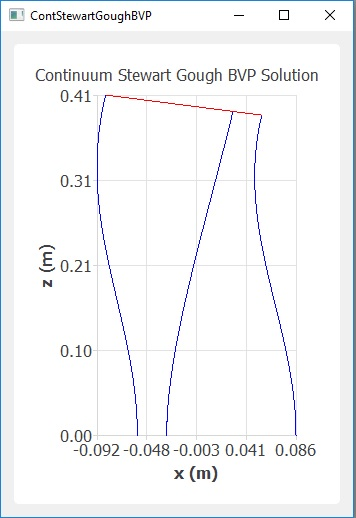
\includegraphics[width=0.50\textwidth]{fig/SolutionPlot.jpg}
	\label{fig:SolutionPlot}
\end{figure}


\end{document}